\chapter{Дифференциальная геометрия кривых}

\section{Вектор-функция}

\begin{remark}
	Все функции, которые будут в курсе, будут предполагаться достаточно гладкими (т. е. нужная производная всегда существует и непрерывна)
\end{remark}

\begin{definition}
	$ f : [a, b] $ (можно считать $ [0, 1] $) $ \to \R^3 $ (непр.; дифф. настолько, насколько нам надо) -- вектор-функция \\
	$ f([a, b]) $ -- кривая; $ f(a) $ -- начало; $ f(b) $ -- конец
\end{definition}

\begin{definition}
	$ A = \liml{t \to t_0} f(t), \quad A \in \R^3 $, если
	$$ \forall \veps > 0 \quad \exist \delta(\veps) > 0 : |t - t_0| < \delta \implies |\vec{f}(t) - A| < \veps $$
\end{definition}

\begin{undefthm}{Операции с вектор-функциями}
	\hfill
	\begin{itemize}
		\item $ \bigg( \vec{f} + \vec{g} \bigg )(t) \define \vec{f}(t) + \vec{g}(t) $
		\item $ (\alpha \cdot \vec{f})(t) = \alpha \vec{f}(t) $
		\item
		\begin{itemize}
			\item $ \vec{f} \cdot \vec{g}(t) = \bigg( \vec{f}(t), \vec{g}(t) \bigg) $ -- скалярное произведение
			\item $ \vec{f} \times \vec{g}(t) = \vec{f}(t) \times \vec{g}(t) $ -- векторное произведение
			\item $ (\vec{f}, \vec{g}, \vec{h})(t) = \bigg( \vec{f}(t), \vec{g}(t), \vec{h}(t) \bigg) $ -- смешанное произведение
		\end{itemize}
		\begin{statement}
			Эти операции перестановочны с пределом:
			$$ \liml{t \to t_0} (f \times g)(t) = \bigg( \liml{t \to t_0}f(t) \bigg) \times \bigg( \liml{t \to t_0}g(t) \bigg) $$
		\end{statement}
		\begin{proof}
			$$ \vec{f}(t) = \bigg( f_1(t), f_2(t), f_3(t) \bigg), \qquad \vec{g}(t) = \bigg( g_1(t), g_2(t), g_3(t) \bigg) $$
			$$ f \times g = ( f_2g_3 - f_3g_2; f_3g_1 - f_1g_3; f_1g_2 - f_2g_1) $$
			\begin{multline*}
				\liml{t \to t_0}(f \times g)(t) \stackrel?= \bigg( \liml{t \to t_0}(f_2g_3 - f_3g_2)(t); \widedots[5em] \bigg) = (\vawe{f_2}\vawe{g_3} - \vawe{f_3}\vawe{g_2}; \widedots[5em]) = \\
				= (\vawe{f_1}; \vawe{f_2}; \vawe{f_3}) \times (\vawe{g_1}; \vawe{g_2}; \vawe{g_3})
			\end{multline*}
			$$ \liml{t \to t_0} \bigg( f_2(t)g_3(t) - g_2(t)f_3(t) \bigg) = \underbrace{\liml{t \to t_0} f_2(t)}_{= \vawe{f_2}} \liml{t \to t_0}g_3(t) - \liml{t \to t_0}(t) \liml{t \to t_0}f_3g_3(t) $$
		\end{proof}
	\end{itemize}
\end{undefthm}

\begin{undefthm}{Почему предел можно брать по координатам?}
	$ f(t) = \bigg( f_1(t); f_2(t); f_3(t) \bigg) $
	$$ \liml{t \to t_0} f(t) = A = (A_1, A_2, A_3) \iff \liml{t \to t_0} f_i(t) = A_i \iff \forall \veps > 0 \quad \exist \delta > 0 : |t - t_0| < \delta \implies |f_i(t) - A_i| < \frac\veps3 $$
\end{undefthm}

\begin{iproof}
	\item $ \impliedby $
	$$ |\vec{f(t)} - A| = \sqrt{\bigg( \underbrace{f_1(t) - A_1}_{< \frac\veps3} \bigg)^2 + \bigg(\underbrace{f_2(t) - A_2}_{< \frac\veps3} \bigg)^2 + \bigg( \underbrace{f_3(t) - A_3}_{< \frac\veps3} \bigg)^2} < \sqrt{\frac{\veps^2}3} < \veps $$
	\item $ \implies $ \\
	Допустим противное:
	$$ \exist \veps_0 : \forall \delta > 0 \quad \exist t_\delta : |t_\delta - t_0| < \delta; \quad |f_1(t_\delta) - A_1| \ge \veps_0 $$
\end{iproof}

\begin{definition}
	$ f(t) $ непр. в $ t_0 $, если $ f(t_0) = \liml{t \to t_0} f(t) $
\end{definition}

\begin{definition}
	$ \vec{f}'(t_0) \define \liml{t \to t_0} \frac{f(t) - f(t_0)}{t - t_0} $
\end{definition}

\begin{stmts}
	\item $ (f + g)' = f' + g' $
	\item $ (\alpha \vec{f})' = \alpha'\vec{f} + \alpha \vec{f}' $
	\item $ (\vec{f}\vec{g})' = \vec{f}'\vec{g} + \vec{f}\vec{g}' $
	\item $ (\vec{f} \times \vec{g})' = \vec{f}' \times \vec{g} + \vec{f} \times \vec{g}' $
	\begin{proof}
		\begin{multline*}
			(f \times g)'(t_0) = \liml{t \to t_0} \frac{f(t) \times g(t) - f(t_0) \times g(t_0)}{t - t_0} = \\
			= \liml{t \to t_0} \frac{f(t) \times g(t) - f(t_0) \times g(t) + f(t_0) \times g(t) - f(t_0) \times g(t_0)}{t - t_0} = \\
			= \liml{t \to t_0} \bigg( \frac{f(t) - f(t_0)}{t - t_0} \times g(t) \bigg) + f(t_0) \times \liml{t \to t_0} \frac{g(t) - g(t_0)}{t - t_0} = f'(t_0) \times g(t_0) + f(t_0) \times g'(t_0)
		\end{multline*}
	\end{proof}
	\item $ (f, g, h)' = (f', g, h) + (f, g', h) + (f, g, h') $
\end{stmts}

\begin{undefthm}{Утверждение, которое не переносится на вектор-функции}
	\begin{theorem}[Лагранжа]
		$ f(b) - f(a) = f'(c)(b - a), \qquad \exist c \in [a, b] $
	\end{theorem}
	Не работает в векторном случае
\end{undefthm}

\begin{lemma}
	$ |\vec{f}| = \const \iff \vec{f}' \perp \vec{f} $
\end{lemma}

\begin{proof}
	$$ |\vec{f}| = \const \iff (\vec{f}, \vec{f}) = \const \iff \frac{\di f}{\di t}(f, f) = 0 \iff 2(f, f') = 0 \iff f \perp f' $$
\end{proof}

\subsection{Параметризация и перепарамаетризация}

$ \vec{f} $ называется параметризацией кривой

\begin{definition}[перепараметризация]
	$ f : [a, b] \to \R^3, \qquad g : [c, d] \to \R^3 $ \\
	$ \vec{f} $ и $ \vec{g} $ -- параметризации одной кривой, если
	$$ \exist \underset{
		\begin{subarray}{c}
			\alpha \text{ непр.} \\
			\alpha(a) = c \\
			\alpha (b) = d \\
			\alpha \text{ строго возрастает}
		\end{subarray}}{\alpha : [a, b] \to [c, d]} : f(t) = g \big( \alpha(t) \big) \quad \forall t \in [a, b] $$
\end{definition}

Кривая $ \equiv $ класс эквиваентности вектор-фукнций

\section{Касательный вектор}

\begin{definition}
	$ \vec{f'}(t_0) $ называется касательным вектором
\end{definition}

\begin{statement}
	$ f \sim g \implies f'(t_0) \parallel g' \big( \alpha(t_0) \big) $
\end{statement}

\begin{proof}
	$$ \vec{f}(t) = \vec{g} \big( \alpha(t) \big) $$
	$$ \vec{f'}(t) = \vec{g'} \big( \alpha(t) \big) \cdot \underbrace{\alpha'(t)}_{> 0} \implies \vec{f}'(t) \upuparrows \vec{g}' \big( \alpha(t) \big) $$
\end{proof}

\begin{definition}
	Касательная -- совокупность касательных векторов и противоположных им и $ \vec{0} $
\end{definition}

\begin{definition}
	Регулярная параметризация -- параметизация с требованием, чтобы $ \vec{f}'(t) \ne \vec{0} \quad \forall t $
\end{definition}

\begin{eg}
	$ f(t) = (t^2, t^3, t^4) $ -- не регулярная
\end{eg}

\begin{definition}
	Кривая называется регулярной, если она допускает регулярную параметризацию
\end{definition}

\begin{theorem}
	$ \delta $ -- расстояние от $ f(t) $ до касательной прямой
	$$ \implies \liml{t \to t_0} \frac\delta{|\vec{f}(t) - \vec{f}(t_0)|} = 0 $$
	Касательная -- единственная прямая, обладающая таким свойством
\end{theorem}

\begin{remark}
	Предел -- синус зелёного угла на рис. \ref{fig:1}
\end{remark}

\begin{figure}[!ht]
	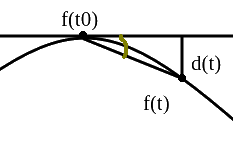
\includegraphics[scale=1]{1}
	\caption{Теорема о касательной}
	\label{fig:1}
\end{figure}

\begin{undefthm}{Уравнение касательной к прямой}
	$$ \vec{v}(t) = \vec{f'}(t_0) \cdot \tau + \vec{f}(t_0) $$
\end{undefthm}

\begin{proof}[теоремы]
	$$ \delta(t) = \frac{\bigg| \bigg( \big( f(t) - f(t_0) \big) \times f'(t_0) \bigg) \times f'(t_0) \bigg|}{|f'(t_0)|^2} $$
	Введём такую систему координат, чтобы касательная была осью $ OX $:
	$$ \vec{f}(t) = \bigg( f_1(t), f_2(t), f_3(t) \bigg) $$
	$$ f'(t) = (1, 0, 0) $$
	$$ f(t_0) = (0, 0, 0) $$
	Посчитаем двойное векторное произведение:
	$$ \bigg( f(t) - f(t_0) \bigg) \times f'(t_0) = \bigg( f_1(t), f_2(t), f_3(t) \bigg) \times (1, 0, 0) = (0, f_3, -f_2) $$
	$$ (0, f_3, -f_2) \times (1, 0, 0) = (0, -f_2, f_3) $$
	$$ \delta = \frac{\sqrt{f_2^2 + f_3^2}}1 $$
	$$ \liml{t \to t_0} \frac{\delta^2}{|f(t) - f(t_0)|^2} = \liml{t \to t_0} \frac{f_2^2(t) + f_3^2(t)}{f_1^2(t) + f_2^2(t) + f_3^2(t)} $$
	Неопределённость -- $ (0, 0, 0) $
	$$ f_1(t_0) = f_2(t_0) = f_3(t_0) $$
	\begin{multline*}
		\lim ... \underset{\text{Лопиталь}}= \liml{t \to t_0} \frac{\cancel2f_2f_2' + \cancel2f_3f_3'}{\cancel2(f_1f_1' + f_2f_2' + f_3f_3')} \underset{\text{Лопиталь}}= \\
		= \liml{t \to t_0} \frac{f_2'^2 + f_2f_2'' + f_3'^2 + f_3f_3''}{\underbrace{f_1'^2} _{\to 1} + \underbrace{f_1f_1'' + f_2'^2 + f_2f_2''}_{\to 0} + \underbrace{f_3'^2}_{\to 0} + \underbrace{f_3f_3''}_{\to 0}} = 0 \iff \vect{f}'(t) \parallel (1, 0, 0)
	\end{multline*}
\end{proof}
